% Made up for the tikra benchmark.
\usetikzlibrary{shapes.arrows}
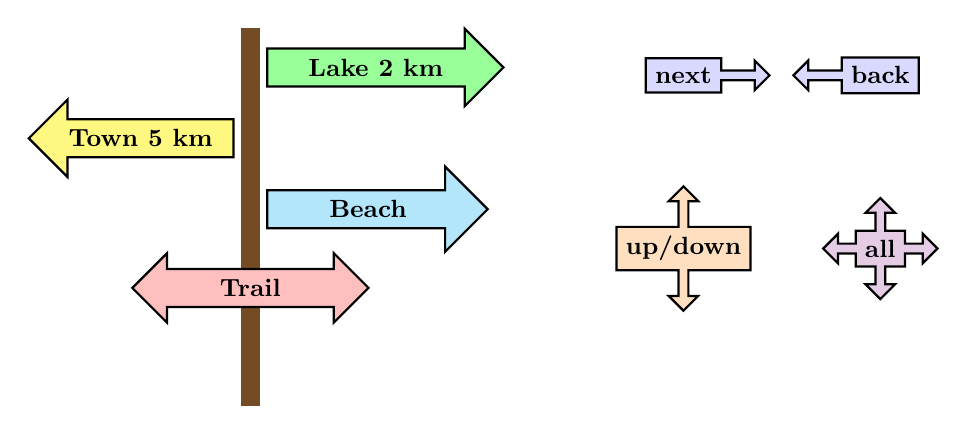
\begin{tikzpicture}[font=\small\bfseries, every node/.style={draw, thick}]
  % a signpost: single arrows pointing at made-up places
  \fill[brown!60!black] (-0.12,-3.2) rectangle (0.12,1.6);
  \node[single arrow, fill=green!40, minimum height=3cm, anchor=west, shape border rotate=0] at (0.2,1.1) {Lake 2 km};
  \node[single arrow, fill=yellow!50, minimum height=2.6cm, anchor=east, shape border rotate=180] at (-0.2,0.2) {Town 5 km};
  \node[single arrow, fill=cyan!30, minimum height=2.8cm, anchor=west, single arrow head extend=3mm] at (0.2,-0.7) {Beach};
  \node[double arrow, fill=red!25, minimum height=3cm, double arrow head extend=2mm] at (0,-1.7) {Trail};
  % arrow boxes
  \node[arrow box, arrow box arrows={east:0.6cm}, fill=blue!15] at (5.5,1) {next};
  \node[arrow box, arrow box arrows={west:0.6cm}, fill=blue!15] at (8,1) {back};
  \node[arrow box, arrow box arrows={north:0.5cm, south:0.5cm}, fill=orange!25] at (5.5,-1.2) {up/down};
  \node[arrow box, arrow box arrows={north:0.4cm, east:0.4cm, south:0.4cm, west:0.4cm}, fill=violet!20] at (8,-1.2) {all};
\end{tikzpicture}
